%include part: see main.beamer.tex and main.article.tex
%include common packages and settings
\usepackage{etex} %эта магическая херь избавляет от переполнения регистров TeX а!!!

\mode<article>{\usepackage{fullpage}}
\mode<presentation>{
    \usetheme{Madrid} %%Boadilla,Madrid,AnnArbor,CambridgeUS,Malmoe,Singapore,Berlin
    \useoutertheme{shadow}
} 

\usepackage[utf8]{inputenc}
\usepackage[russian]{babel}
\usepackage{indentfirst}
\usepackage{graphicx}

\usepackage{amsmath}
\usepackage{amsfonts}
\usepackage{amsthm}
\usepackage{algorithm}
\usepackage{algorithmic}

\usepackage[all]{xy}

\date{Лекция по дисциплине <<дискретная математика>>\\(\today)}
\author[М.~М.~Шихов]{Михаил Шихов \\ \texttt{\underline{m.m.shihov@gmail.com}}}

%для рисования графов пакетом xy-pic
\entrymodifiers={++[o][F-]}

%для псевдокода алгоритмов (algorithm,algorithmic)
\renewcommand{\algorithmicrequire}{\textbf{Вход:}}
\renewcommand{\algorithmicensure}{\textbf{Выход:}}
\renewcommand{\algorithmiccomment}[1]{// #1}
\floatname{algorithm}{Псевдокод}



\title[Индукция и рекурсия]{Индукция и рекурсия}


\begin{document}

%титул и содержание статьи
\mode<article>{\maketitle\tableofcontents}

%титул и содержание презентации
\frame<presentation>{\titlepage}
\begin{frame}<presentation>
    \frametitle{Содержание}
    \tableofcontents
\end{frame}


Чтобы понять что такое \emph{рекурсия}, нужно понять, что такое \emph{рекурсия}. 


\section{Индукция и рекурсия}

Термины \emph{индукция} и \emph{рекурсия} часто употребляются вместе. Следует провести границу между ними.


\subsection{Индукция}

Математическая \emph{индукция} --- это метод рассуждений (доказательства) от частного к общему. То есть утверждения об общем случае выводятся(\emph{индуцируются}) из очевидных частных случаев --- \emph{фактов}. Базовый принцип математической индукции заключается в следующем.

\begin{frame}
    \frametitle{Базовый принцип математической индукции}
    
    \begin{enumerate}
        \item<1-> \emph{Базис}. Показана истинность утверждения $P(i)$, где $i\in\mathbb{N}$. Обычно $i=0$ или $i=1$. Но в общем случае может быть и так, что $P(j)$ ложно для $j<i$.
        \item<2-> \emph{Индуктивный переход}. Для произвольного $n\geq i,n\in\mathbb{N}$ доказано, что из истинности $P(n)$ следует истинность $P(n+1)$. Т.е. доказываем $P(n)\Rightarrow P(n+1)$.
    \end{enumerate}
\end{frame}

\begin{frame}[allowframebreaks]
    \frametitle{Пример}
    \begin{example}
        Задача. Доказать, что 
        \[
            \sum_{i=0}^{n}i^2=\frac{2n^3+3n^2+n}{6}.
        \]
    \end{example}
    \begin{proof}[Решение]
        База: при $n=0$ равенство выполняется.
        
        Индуктивный переход: $n\geq 0$.  $P(n+1)$:
        \[
            \sum_{i=0}^{n+1}i^2=\frac{2n^3+9n^2+13n+6}{6}.
        \]
        $P(n)\Rightarrow P(n+1)$:
        \[
            \begin{split}
                \sum_{i=0}^{n+1}i^2=(n+1)^2+\sum_{i=0}^{n}i^2=\\
                =(n+1)^2+\frac{2n^3+3n^2+n}{6}=\frac{2n^3+9n^2+13n+6}{6}.
            \end{split}
        \]
        Следовательно, доказываемое утверждение спрведливо для всех $n$.
    \end{proof}
\end{frame}

Общая форма математической индукции заключается в следующем.
\begin{frame}
    \frametitle{Общая форма математической}
    \begin{enumerate}
        \item<1-> \emph{Базис}. Показана истинность утверждений $P(i),P(i+1),\ldots,P(j)$, где $i,j\in\mathbb{N},j>i$.
        \item<2-> \emph{Индуктивный переход}. Для $n\geq j$ при доказательстве истинности $P(n+1)$ можно использовать не только $P(n)$, но и все утверждения $P(i),P(i+1),\ldots,P(n)$.
    \end{enumerate}
\end{frame}

\begin{frame}[allowframebreaks]
    \frametitle{Пример}
    \begin{example}
        Задача. Доказать $P(n)$: если $n\geq 8$, то $n$ можно представить суммой троек и пятерок.
    \end{example}
    \begin{proof}[Решение]
            Базис: $8=3+5, 9=3+3+3, 10=5+5$. 
            
            Индуктивный переход. Предполагаем истинность $P(8),P(9),P(10),\ldots,P(n)$. Доказывая $P(n+1)$ вычтем $3$ из $n+1$. Заметим, что $P(n-2)$ истинно. То есть $n-2$ представимо суммой $3k+5m$ пятерок и троек, а стало быть и $n+1$ также представимо, так как $n+1=3(k+1)+5m$.
    \end{proof}
\end{frame}


\subsection{Рекурсия}

\begin{frame}
    \frametitle{Рекурсия}
    \begin{definition}
        \alert{Рекурсия} в общем случае --- это \emph{самоподобие}. 
    \end{definition}
    
    Таким свойством самоподобности, кроме всех прочих объектов, могут обладать
    \begin{itemize}
        \item математические формулы, 
        \item данные 
        \item алгоритмы. 
    \end{itemize}
\end{frame}

Примером рекурсивной (самоподобной) структуры данных может быть список.

\begin{frame}
    \frametitle{Рекурсивное определение структуры данных \alert{список}}
    \begin{example} 
        Пусть имеются атомарные (неделимые) типы данных, такие как: число, строка, символ и т.д. Список можно определить так:
        \begin{enumerate}
            \item любой атом есть \alert{список};
            \item если $l_1,l_2,\ldots,l_n$ --- списки, то $(l_1,l_2,\ldots,l_n)$ есть \alert{список};
            \item ничто другое не является списком.
        \end{enumerate}
        
        Вариант списка: $(1,(2,(3,4)),5)$.\qed
    \end{example}
\end{frame}

Рекурсивный алгоритм решения задачи обычно выполняется так:
\begin{frame}
    \frametitle{Шаблон рекурсивного алгоритма решения задачи}
    \begin{enumerate}
        \item<1-> если задача \alert<1>{тривиальна}, то выдается решение и алгоритм завершается;
        \item<2-> в противном случае исходная задача разбивается на \alert<2>{подзадачи} меньшей размерности;
        \item<3-> каждая \alert<3>{подзадача}, решается тем же алгоритмом, что и исходная задача (то есть \emph{рекурсивно});
        \item<4-> решения \alert<4>{подзадач} объединяются так, чтобы получить решение исходной \alert<4>{задачи}.
    \end{enumerate}
\end{frame}

Важно отметить следующие особенности рекурсивных алгоритмов.
\begin{frame}
    \frametitle{Особенности рекурсивных алгоритмов}
    \begin{enumerate}
        \item Существование одного или нескольких \alert{базовых} случаев для решаемой задачи. Решение базового случая тривиально и может быть получено сразу. Именно к базовым случаям в конечном итоге сводится решение любой исходной задачи.
        
        \item Существование \alert{способа сведения} исходной задачи к решению подобных ей подзадач и получения результата исходной задачи на основе результатов подзадач.
    \end{enumerate}
\end{frame}


\subsection{Рекурсивные вычисления}

\begin{frame}
    \frametitle{Вычисление факториала числа $n$}
    \framesubtitle{Классический неудачный пример рекурсии}
    
    \begin{algorithm}[H]
        \caption{factorial($n$)}
        \begin{algorithmic}[1]
            \REQUIRE{$n\in\mathbb{N}$}
            \ENSURE{$n!$}
            
            \IF{$n=0$}
                \RETURN{$1$}
            \ELSE
                \RETURN{$n$ $\cdot$ factorial($n-1$)}
            \ENDIF
        \end{algorithmic}
    \end{algorithm}
\end{frame}

\begin{frame}
    \frametitle{Вычисление факториала числа $n$}
    \framesubtitle{В итеративной форме поиск факториала выглядит намного проще}
    
    \begin{algorithm}[H]
        \caption{factorial($n$)}
        \begin{algorithmic}[1]
            \REQUIRE{$n\in\mathbb{N}$}
            \ENSURE{$n!$}
            \STATE{$r\gets 1$}
            \WHILE{$n\geq 1$}
                \STATE{$r\gets r\cdot n$}
                \STATE{$n\gets n-1$}
            \ENDWHILE
            \RETURN{$r$}
        \end{algorithmic}
    \end{algorithm}
    Вычисление факториала --- это хороший пример бессмысленной задачи
\end{frame}

\begin{frame}
    \frametitle{Вычисление $n$-го числа Фибоначчи}
    \framesubtitle{Рекурсивный алгоритм}
    
    \begin{algorithm}[H]
        \caption{fib($n$)}
        \begin{algorithmic}[1]
            \REQUIRE{$n\in\mathbb{N}$ --- номер числа Фибоначчи}
            \ENSURE{$n$-е число Фибоначчи}
            
            \IF{$n=0$}
                \RETURN{$0$}
            \ENDIF
            \IF{$n=1$}
                \RETURN{$1$}
            \ENDIF
            \RETURN{fib($n-1$) + fib($n-2$)}
        \end{algorithmic}
    \end{algorithm}
\end{frame}

\begin{frame}
    \frametitle{Вычисление $n$-го числа Фибоначчи}
    \framesubtitle{В итеративной форме выглядит проще}
    
    \begin{algorithm}[H]
        \caption{fib($n$)}
        \begin{algorithmic}[1]
            \REQUIRE{$n\in\mathbb{N}$ --- номер числа Фибоначчи}
            \ENSURE{$n$-е число Фибоначчи}
            
            \STATE{$i\gets 0$}
            \STATE{$F_{0}\gets 0$}
            \STATE{$F_{1}\gets 1$}
            \WHILE{$i<n$}
                \STATE{$i\gets i+1$}
                \STATE{$t\gets F_{1}$}
                \STATE{$F_{1}\gets F_{1} + F_{0}$}
                \STATE{$F_{0}\gets t$}
            \ENDWHILE
            \RETURN{$F_{0}$}
        \end{algorithmic}
    \end{algorithm}
\end{frame}

\begin{frame}
    \begin{center}Пример поиска суммы\end{center}
    
    \begin{algorithm}[H]
        \caption{$s(n)$}
        \begin{algorithmic}[1]
            \STATE{$s\gets 0$}
            \STATE{$i\gets 1$}
            \WHILE{$i\leq n$}
                \STATE{$s\gets s+i$}
                \STATE{$i\gets i+1$}
            \ENDWHILE
            \RETURN{$s$}
        \end{algorithmic}
    \end{algorithm}
    \begin{center}можно выразить рекурсивными алгоритмами...\end{center}
\end{frame}
    
\begin{frame}
    \begin{algorithm}[H]
        \caption{$s(n)$}
        \begin{algorithmic}[1]
            \RETURN{$\texttt{doWhileIter}(1,n,0)$}
            \COMMENT{или $\texttt{doWhileRec}(1,n)$}
        \end{algorithmic}
    \end{algorithm}
    
    \begin{algorithm}[H]
        \caption{$\texttt{doWhileIter}(i, n, s)$}
        \begin{algorithmic}[1]
            \IF{$i\leq n$}
                \RETURN{$\texttt{doWhileIter}(i+1, n, s+i)$}
            \ENDIF
            \RETURN{$s$}
        \end{algorithmic}
    \end{algorithm}
    
    \begin{algorithm}[H]
        \caption{$\texttt{doWhileRec}(i, n)$}
        \begin{algorithmic}[1]
            \IF{$i\leq n$}
                \RETURN{$i+\texttt{doWhileRec}(i+1, n)$}
            \ENDIF
            \RETURN{$n$}
        \end{algorithmic}
    \end{algorithm}
\end{frame}
    
\begin{frame}
    \frametitle{Задача о размене}
    \begin{example}
        Сколько существует вариантов размена суммы в один рубль монетами, достоинством по 5, 10, 15, 20, 25 и 50 копеек?
    \end{example}
\end{frame}

\begin{frame}
    \frametitle{Задача о размене}
    \framesubtitle{Решение}
    
    \begin{algorithm}[H]
        \caption{$sс(s, ct)$}
        \begin{algorithmic}[1]
            \REQUIRE{$s$ --- размениваемая сумма; $ct$ --- тип монеты (натуральное число); $value(ct)$ --- достоинство монеты типа $ct$}
            \ENSURE{Количество вариантов размена}
            
            \IF{$s=0$}
                \RETURN{$1$}
            \ELSIF{$s<0$ \OR $ct\leq 0$}
                \RETURN{$0$}
            \ELSE
                \RETURN{$sc(s,ct-1) + sc(s-value(ct), ct)$}
            \ENDIF
        \end{algorithmic}
    \end{algorithm}
\end{frame}

\begin{frame}
    \begin{algorithm}[H]
        \caption{$value(ct)$}
        \begin{algorithmic}[1]
            \REQUIRE{$ct$ --- тип монеты (натуральное число);}
            \ENSURE{Достоинство монеты типа $ct$}
            
            \IF{$ct=0$}
                \STATE{\textbf{halt()}}
            \ELSIF{$ct=1$}
                \RETURN{$1$}
            \ELSIF{$ct=2$}
                \RETURN{$2$}
            \ELSIF{$ct=3$}
                \RETURN{$3$}
            \ELSIF{$ct=4$}
                \RETURN{$5$}
            \ELSE
                \STATE{\textbf{halt()}}
            \ENDIF
        \end{algorithmic}
    \end{algorithm}
\end{frame}


\section{Реккурентные математические формулы}

Выражающиеся сами через себя математические формулы называют \emph{реккурентными}. Вычисление значений таких формул для больших $n$ занимает слишком много времени, поэтому представляет интерес возможность свести реккурентность к <<замкнутой>> (аналитической) формуле, то есть к вычислимой непосредственно. Для рассматриваемых ниже реккурентных формул первого и второго рода порой удается получить решение в <<замкнутой форме>>.


\subsection{Реккурентные формулы первого рода}

В качестве примера рассмотрим задачу о Ханойских башнях.
\begin{frame}
    \frametitle{Задача о Ханойских башнях}

    \begin{example}[Задача о Ханойских башнях]
        На первый из трех алмазных стержней насажены золотые диски в количестве 64-х штук. Все диски разного диаметра и диск меньшего диаметра лежит на диске большего диаметра. Требуется переместить диски на третий стержень в том же порядке, в каком они находятся на первом, перекладывая за раз по одному диску. Второй столбик используется как вспомогательный. В процессе перемещения нельзя класть больший диск на меньший\footnote{По легенде задача поставлена Всевышним перед жрецами, которые в настоящий момент над ней должны работать в несколько смен днем и ночью, и как только они закончат, наступит конец света. Хотелось бы прикинуть: стоит ли вообще браться за дальнейшее изучение рекурсии?}.
    \end{example}
\end{frame}

\begin{frame}[allowframebreaks]
    \frametitle{Решение задачи о Ханойских башнях}
    
    Возьмем меньшее количество дисков и убедимся, что задача решаема:
    \[
    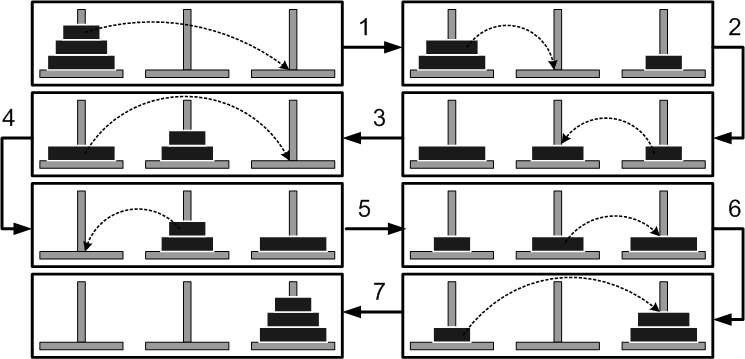
\includegraphics[width=0.57\textwidth]{fig/hanoi.png}
    \]
    Для одного диска решение очевидно. Для двух тоже.

    Попробуем обобщить на произвольное количество дисков. Для того, чтобы перенести $n$ дисков на третий столбик нужно $n-1$ верхних дисков сложить на второй столбик (очевидно, это можно сделать), оставшийся на первом столбике диск переложить на третий, и на него переместить $n-1$ дисков со второго:

    \[
    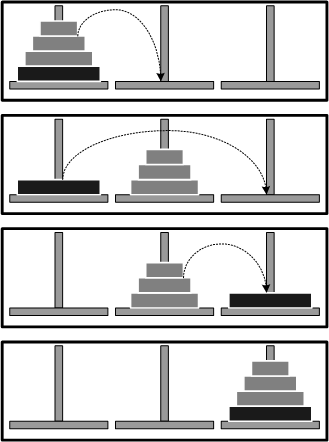
\includegraphics[width=0.27\textwidth]{fig/hanoi4.png}
    \]

    Стало быть, если $T(n)$ --- количество перекладываний для переноса $n$ дисков, имеем: перенос на второй столбик потребует $T(n-1)$ перекладываний, одно перекладывание с первого на третий, и финальные $T(n-1)$ перекладываний на третий. $T(n)=2\cdot T(n-1) + 1$. В реккурентной форме (обобщив для 0 дисков):
    \[
        T(n)=
        \begin{cases}
            0,                  & n=0, \text{\emph{База рекурсии}},\\
            2\cdot T(n-1) + 1,  & n>0, \text{\emph{Реккурентный переход}}.
        \end{cases}
    \]

    Теперь можно легко двигаться от базы, получая:
    \[
        \begin{array}[c]{c||c|c|c|c|c|c|c|c|c|}
            \hline
            n       &0  &1  &2  &3  &4  &5  &6  &7   &8\\ \hline
            T(n)    &0  &1  &3  &7  &15 &31 &63 &127 &255\\ \hline
        \end{array}
    \]

    Тем не менее это неудобно --- слишком много последовательных решений. Хотелось бы сразу, не впадая в рекурсивный спуск, ответить сколько же нужно перекладываний для перемещения $n$ дисков? Пусть $K(n)=T(n)+1$.

    \[
        \begin{split}
                        T(n)+1=2\cdot T(n-1) + 2\Rightarrow\\
            \Rightarrow T(n)+1=2\cdot (T(n-1) + 1)\Rightarrow\\
            \Rightarrow K(n)=2\cdot (K(n-1))\Rightarrow\\
            \Rightarrow K(n)=2\cdot 2\cdot (K(n-2))\Rightarrow\\
            \Rightarrow K(n)=\underbrace{2\cdot 2\cdot\ldots\cdot 2\cdot2}_{n}\cdot K(0) = 2^n\Rightarrow\\
            \Rightarrow T(n)=K(n)-1=2^n-1.
        \end{split}
    \]

    Решением будет\footnote{Возвращаясь к теме конца света: если Всевышний запретил жрецам использовать роботов, то шанс разобраться с рекурсией есть}: $T(64)=2^{64}-1$.
\end{frame}

К сожалению, не всегда получается перейти от реккурентной формулы к простой аналитической, как это сделано в задаче о Ханойских башнях. В общем случае реккурентные формулы первого рода определяются так:
\begin{frame}
    \frametitle{Общий случай реккурентных формул первого рода}
    
    \[
        T(n)=
        \begin{cases}
            f(k),                  & n=k, \text{\emph{База рекурсии}},\\
            c\cdot T(n-1) + f(n),  & n>k, \text{\emph{Реккурентный переход}},
        \end{cases}
    \]
    где $n,k\in\mathbb{N}$, $c$ --- константа, а $f$ --- ненулевая функция от $n$ при $n\geq k$.

    \uncover<2->{
        При этом данной формуле эквивалентна \alert{сумма}:
        \[
            T(n)=\sum_{i=k}^{n}c^{n-i}\cdot f(i).
        \]
    }
\end{frame}

Это можно доказать по индукции, или выполнив $n-k$ подстановок вместо $T(n-1)$ в выражении реккурентного перехода формулы \eqref{eq:rec:rec1type}. Программисту эта эквивалентность дает возможность уйти от рекурсивной подпрограммы к обычному циклу.


\subsection{Реккурентные формулы второго рода}

Примером реккурентных формул второго рода являются числа Фибоначчи, определяемые рекурсивно так:
\begin{frame}
    \frametitle{Числа фибоначчи}
    \begin{example}
    \[
        f(n)=
        \begin{cases}
            0,              &n=0\\
            1,              &n=1\\
            f(n-1)+f(n-2),  &n\geq 2.
        \end{cases}
    \]
    \end{example}
\end{frame}

В общем случае реккурентные формулы второго рода имеют вид
\begin{frame}
    \frametitle{Общий случай реккурентных формул второго рода}
    \[
        f(n)=
        \begin{cases}
            a_{k},                          &n=k\\
            a_{k+1},                        &n=k+1\\
            b_1\cdot f(n-1)+b_2\cdot f(n-2),&n\geq k+2,
        \end{cases}
    \]
    где $b_1,b_2$ --- константы.
\end{frame}

Алгоритм получения аналитического решения для данных соотношений следующий.

\begin{frame}[allowframebreaks]
    \frametitle{Общий случай реккурентных формул второго рода}
    
    \begin{enumerate}
        \item Предположив $f(n)=c^n$, подставить выражение в формулу реккурентного перехода $f(n)=b_1\cdot f(n-1)+b_2\cdot f(n-2)$: 
        \[
            \begin{split}
                            c^n-b_1\cdot c^{n-1}-b_2\cdot c^{n-2} = 0\Rightarrow\\
                \Rightarrow c^{n-2}\cdot(c^2 - b_1\cdot c - b_2) = 0.
            \end{split}
        \]
        
        \item Решить\footnote{Напомним, что для квадратного уравнения $ax^2+bx+c=0$ решениями будут $x_{1,2}=\frac{-b\pm\sqrt{b^2-4ac}}{2a}$} характеристическое уравнение $c^2 - b_1\cdot c - b_2 = 0$ относительно $c$, получив корни $c_1,c_2$.
        
        \item $f(n)$ будет имет следующее аналитическое выражение:
        \begin{equation}
            \label{eq:rec:rec2typeAnalytic}
            f(n)=D_1\cdot {c_1}^n + D_2\cdot{c_2}^n,
        \end{equation}
        где $D_1,D_2$ --- параметры, которые необходимо найти.
        
        \item Воспользоваться начальными условиями, чтобы построить систему уравнений
        \[
            \begin{cases}
                a_k     = D_1\cdot {c_1}^k + D_2\cdot{c_2}^k\\
                a_{k+1} = D_1\cdot {c_1}^{k+1} + D_2\cdot{c_2}^{k+1}\\            
            \end{cases}
        \]
        
        Решить систему относительно двух неизвестных $D_1,D_2$.
        
        \item Решением реккурентности будет формула \eqref{eq:rec:rec2typeAnalytic}.
    \end{enumerate}
\end{frame}

\begin{frame}[allowframebreaks]
    \frametitle{Числа Фибоначчи в аналитическом виде}

    \begin{example}
        Найти аналитическое решение для поиска чисел Фибоначчи.
        \[
            f(n)=
            \begin{cases}
                0,              &n=0\\
                1,              &n=1\\
                f(n-1)+f(n-2),  &n\geq 2.
            \end{cases}
        \]
    \end{example}
    \begin{proof}[Решение] 
        Применяя алгоритм:
        
        \begin{enumerate}
            \item Характеристическое уравнение $c^2-c-1=0$.
            \item Корни характеристического уравнения: $c_1=\frac{1+\sqrt{5}}{2},c_2=\frac{1-\sqrt{5}}{2}$
            \item Решая систему уравнений:
            \[
                \begin{cases}
                    0=D_1 + D_2\\
                    1=D_1\frac{1+\sqrt{5}}{2} + D_2\frac{1-\sqrt{5}}{2},
                \end{cases}
            \]
            получаем решения $D_1=\frac{1}{\sqrt{5}}, D_2=-\frac{1}{\sqrt{5}}$.
            \item Получено $f(n)=\frac{1}{\sqrt{5}}(\frac{1+\sqrt{5}}{2})^n-\frac{1}{\sqrt{5}}(\frac{1-\sqrt{5}}{2})^n$. Следовательно $n$-е число Фибоначчи можно найти, не прибегая к рекурсии.
        \end{enumerate}
    \end{proof}
\end{frame}


\section{Рекурсивные структуры данных и вычисления}


\subsection{Деревья}

\emph{Дерево} --- частный случай графа, может быть определено рекурсивно.

\begin{frame}
    \frametitle{Рекурсивное определение структуры \alert{дерево}}
    \begin{enumerate}
        \item<1-> Одиночный узел $v$ есть дерево, и $v$ является корнем полученного дерева.
        \item<2-> Если $t_1,t_2,\ldots,t_n$ --- деревья, а $v$ одиночный узел, то в результате соединения корня каждого из деревьев $t_1,t_2,\ldots,t_n$ с узлом $v$ будет получено дерево с корнем $v$.
        \item<3-> других правил образования дерева нет.
    \end{enumerate}
\end{frame}

По соглашению будем рисовать дерево так, чтобы корень располагался выше остальных узлов дерева. Дерево настолько универсальная структура, что им можно представить практически любой рекурсивно определяемый объект.

\begin{frame}[allowframebreaks]
    \frametitle{Представление формул деревьями}
    \begin{example} Задача.
        Математическую формулу, состоящую из литералов (чисел), имен переменных и знаков арифметических опереций (например, $+$, $*$) можно определить рекурсивно.
        \begin{enumerate}
            \item Отдельный литерал есть математическая формула.
            \item Отдельное имя переменной есть математическая формула.
            \item Если $A$ и $B$ --- математические формулы, то и $(A+B)$ и $(A*B)$ --- математические формулы.
        \end{enumerate}
        Построить деревья, соответствующие выражениям $1+2*3$ и $(1+2)*3$.
    \end{example}
    
    Решение.
    
    Дерево, соответствующее формуле будем строить так:
    \begin{enumerate}
        \item Отдельному литералу сопоставляется дерево из одного узла (корня), который содержит литерал.
        \item Отдельному имени переменной сопоставляется дерево из одного узла (корня), который содержит имя переменной.
        \item Если $A$ и $B$ --- математические формулы, которым соответствуют деревья $T_A$ и $T_B$, то
        формуле $(A+B)$ соответствует дерево с узлом (корнем) $v$, который содержит символ $+$ и соединяется с корнями деревьев $T_A$ и $T_B$. Дерево для формулы $(A*B)$ определяется аналогично.
    \end{enumerate}
    
    \[
    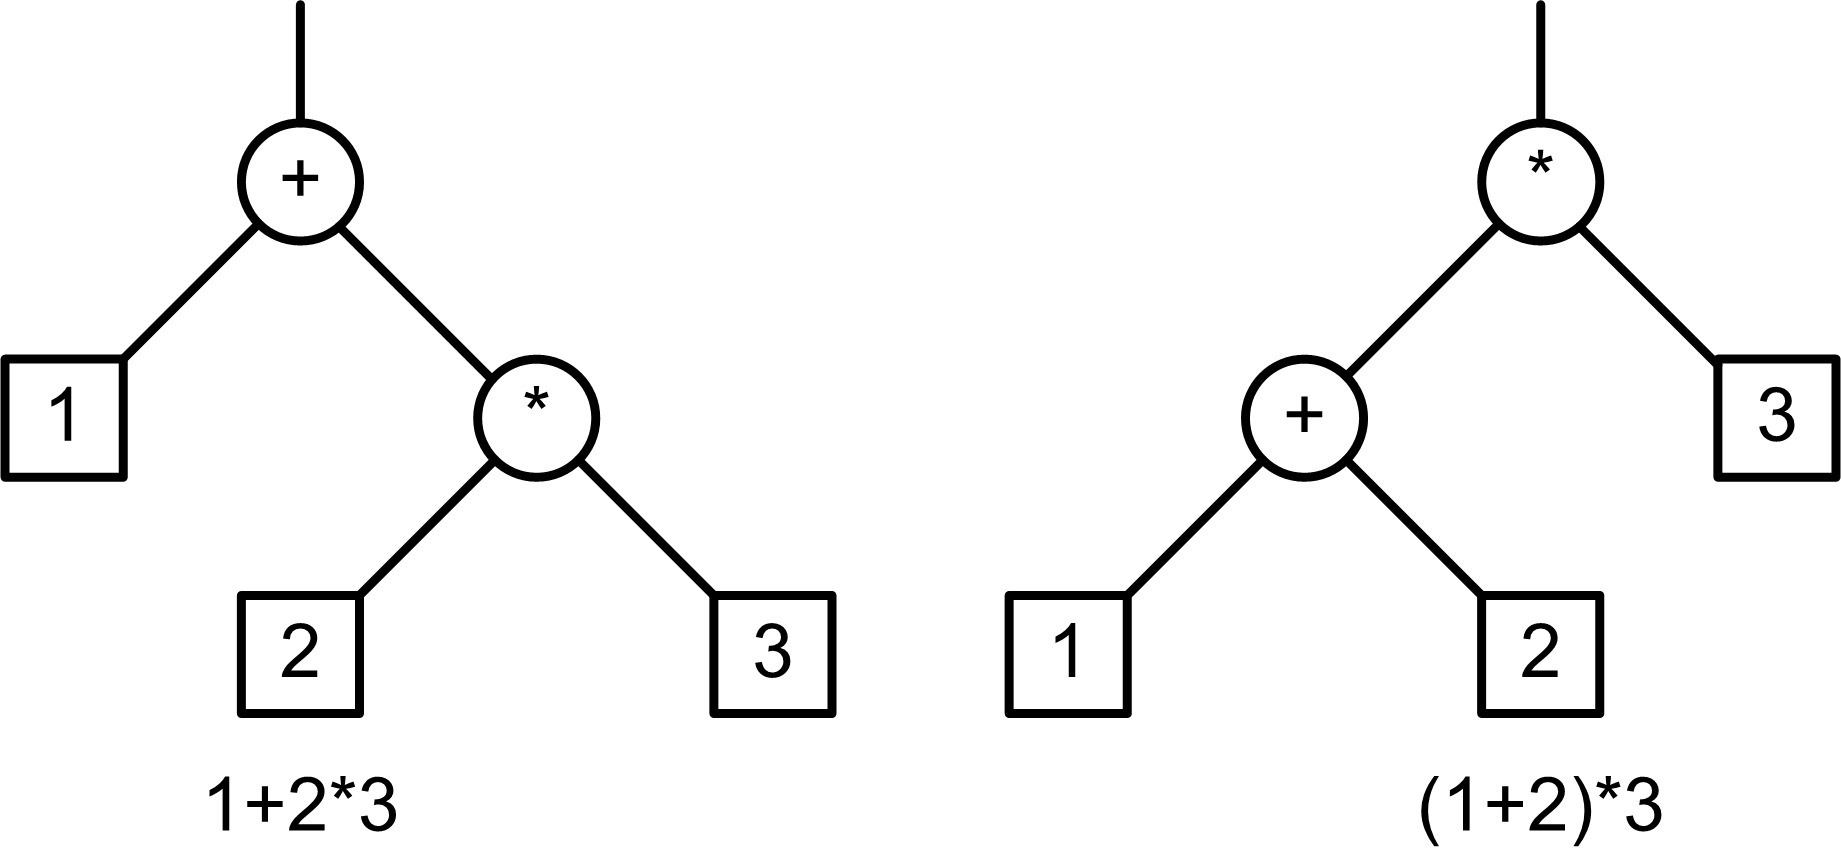
\includegraphics[width=0.67\textwidth]{fig/formulaeTree.png}
    \]
    
    Так как по принятым соглашениям умножение выполняется раньше, то формуле $1+2*3$ эквивалентна формула $(1+(2*3))$, а формуле $(1+2)*3$ --- формула $((1+2)*3)$.
\end{frame}

Привычная запись формул называется \emph{инфиксной}. Проводить вычисления по инфиксной записи не удобно: на порядок действий влияют, например, приоритет, скобки и ассоциативнось операций. Более удобной для вычислений является запись \emph{постфиксная} запись\footnote{Постфиксную запись часто называют польской записью}, не содержащая ни скобок, ни других условностей. Получение постфиксной записи формулы из соответствующего дерева приведено в следующем псевдокоде. Псевдокод для инфиксной и постфиксной форм будет отличаться лишь в строке \ref{alg:l:rec:sOrder}.
\begin{itemize}
    \item Для инфиксной формы: $s\gets \text{<<(>>}s_1s_3s_2\text{<<)>>}$.
    \item Для префиксной формы: $s\gets s_3s_1s_2$.
\end{itemize}


\subsection{Префиксная, инфиксная и постфиксная запись}

\begin{frame}
    \frametitle{Постфиксная запись формулы $postfix(t)$}
    \framesubtitle{Получение по дереву}
    
    \begin{algorithmic}[1]
        \REQUIRE{$t$ --- дерево, соответствующее формуле. $t.text$ --- содержимое узла, $t.left$ --- левое поддерево, $t.right$ --- правое поддерево}
        \ENSURE{$s$ --- постфиксная запись формулы}

        \IF{$t$ --- отдельный узел}
            \STATE{$s\gets t.text$}
        \ELSE[$t$ содержит поддеревья]
            \STATE{$s_1\gets postfix(t.left)$} 
            \STATE{$s_2\gets postfix(t.right)$}
            \STATE{$s_3\gets t.text$}
            \STATE{$s\gets s_1s_2s_3$}\label{alg:l:rec:sOrder}
        \ENDIF
        \RETURN{$s$}
    \end{algorithmic}    
\end{frame}

\begin{frame}
    \frametitle{Обход дерева}
    \framesubtitle{Рекурсивный обход дерева формулы $1+2*3$ и получение префиксной, инфиксной и постфиксной форм.}

    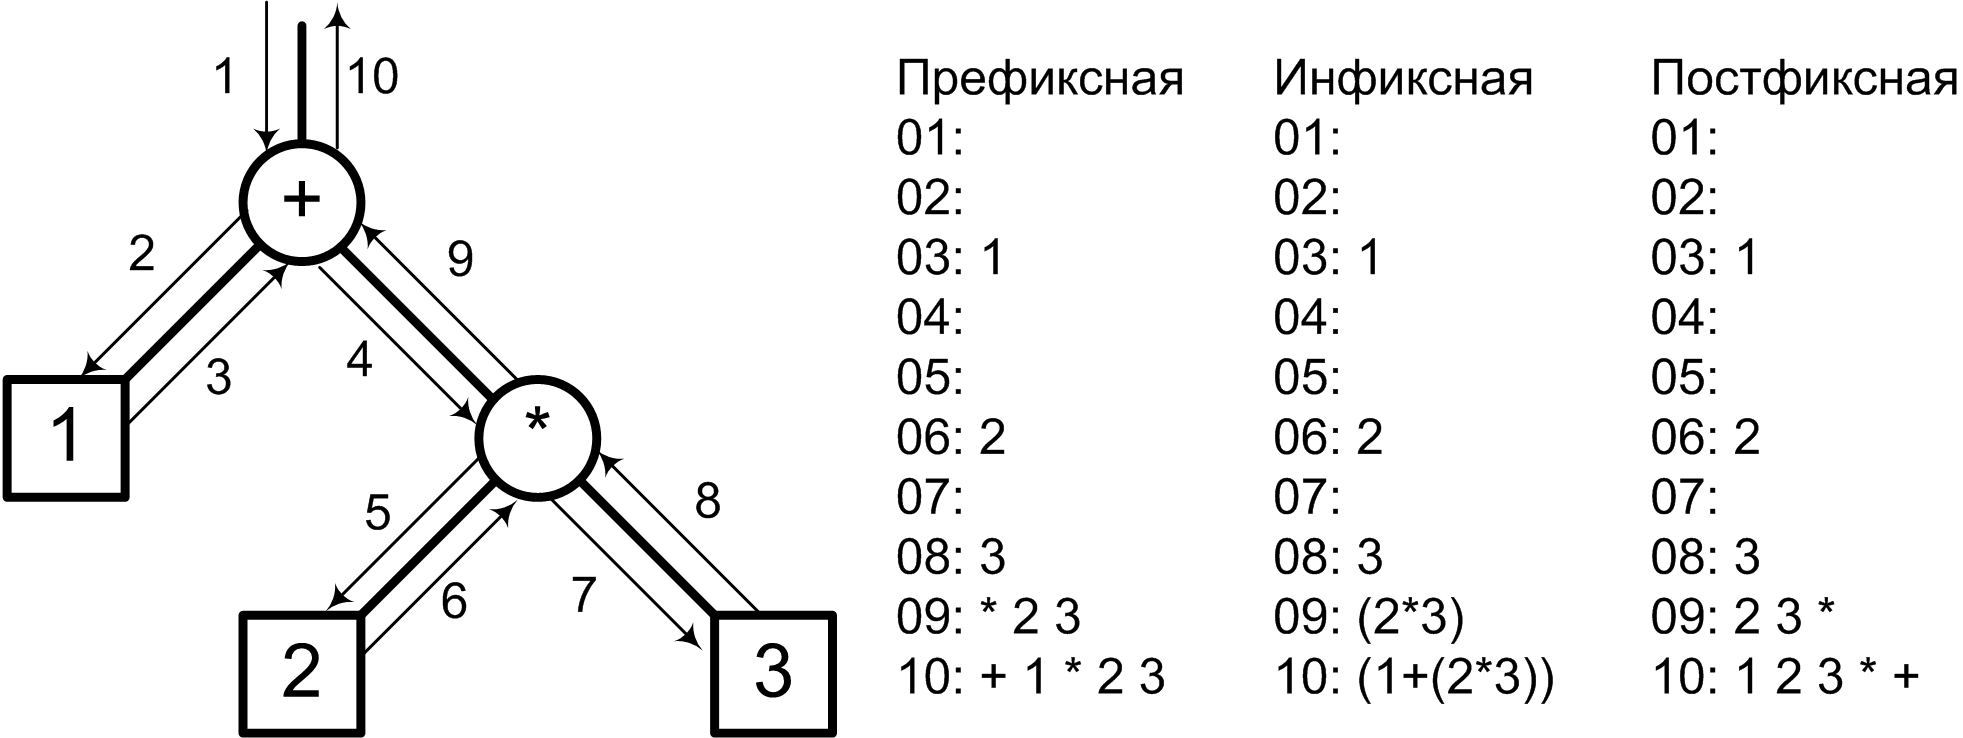
\includegraphics[width=0.87\textwidth]{fig/XfixForms.png}
\end{frame}


\subsection{Стековая машина}

С вычислением постфиксной записи формулы спрвляется \emph{стековая машина}. \emph{Стек} --- это магазинная память, доступ к которой осуществляется с помощью двух команд:
\begin{enumerate}
    \item $push(X)$ --- поместить значение $X$ на вершину стека;
    \item $pop()$ --- изьять с вершины стека значение и вернуть его; $Y=pop()$ --- в $Y$ получим значение с вершины стека.
\end{enumerate}

Стек работает по принципу <<последним пришел, первым ушел>> (LIFO --- Last In First Out). То есть элементы, помещенные в стек командами $push$ будут извлечены в обратном порядке командами $pop$.

Алгоритм работы стековой машины для интерпретации постфиксной записи будет таким.
\begin{frame}
    \frametitle{Алгоритм работы стековой машины}
    \framesubtitle{Интерпретация постфиксной записи}
    \begin{itemize}
        \item Вход: программа в виде выражения в постфиксной записи.
        \item Выход: результат вычисления выражения.
        \item Шаги.
        \begin{enumerate}
            \item Начать просмотр выражения слева направо.
            \item \label{en:rec:stackSee}Встретив число или идентификатор переменной (обозначим и то и другое $X$), поместить значение в стек: $push(X)$, продвинуться на символ влево и перейти на шаг \ref{en:rec:stackSee}. Иначе к следующему шагу.
            \item Если текущий символ выражения --- символ операции, изъять из стека командами $pop()$ необходимое количество аргументов, выполнить соответствующую операцию и поместить результат $R$ в стек $push(R)$. Продвинуться на символ влево и перейти на шаг \ref{en:rec:stackSee}. Иначе к следующему шагу.
            \item Если достигнут конец выражения, то на вершине стека получен результат: $R=pop()$ и завершение алгоритма, иначе перейти на шаг \ref{en:rec:stackSee}.
        \end{enumerate}
    \end{itemize}
\end{frame}

Работа стековой машины проиллюстрирована на рисунке \ref{fig:rec:stackMachine}.

\begin{frame}
    \frametitle{Пример работы стековой машины ($1+2*3$)}
    \[
    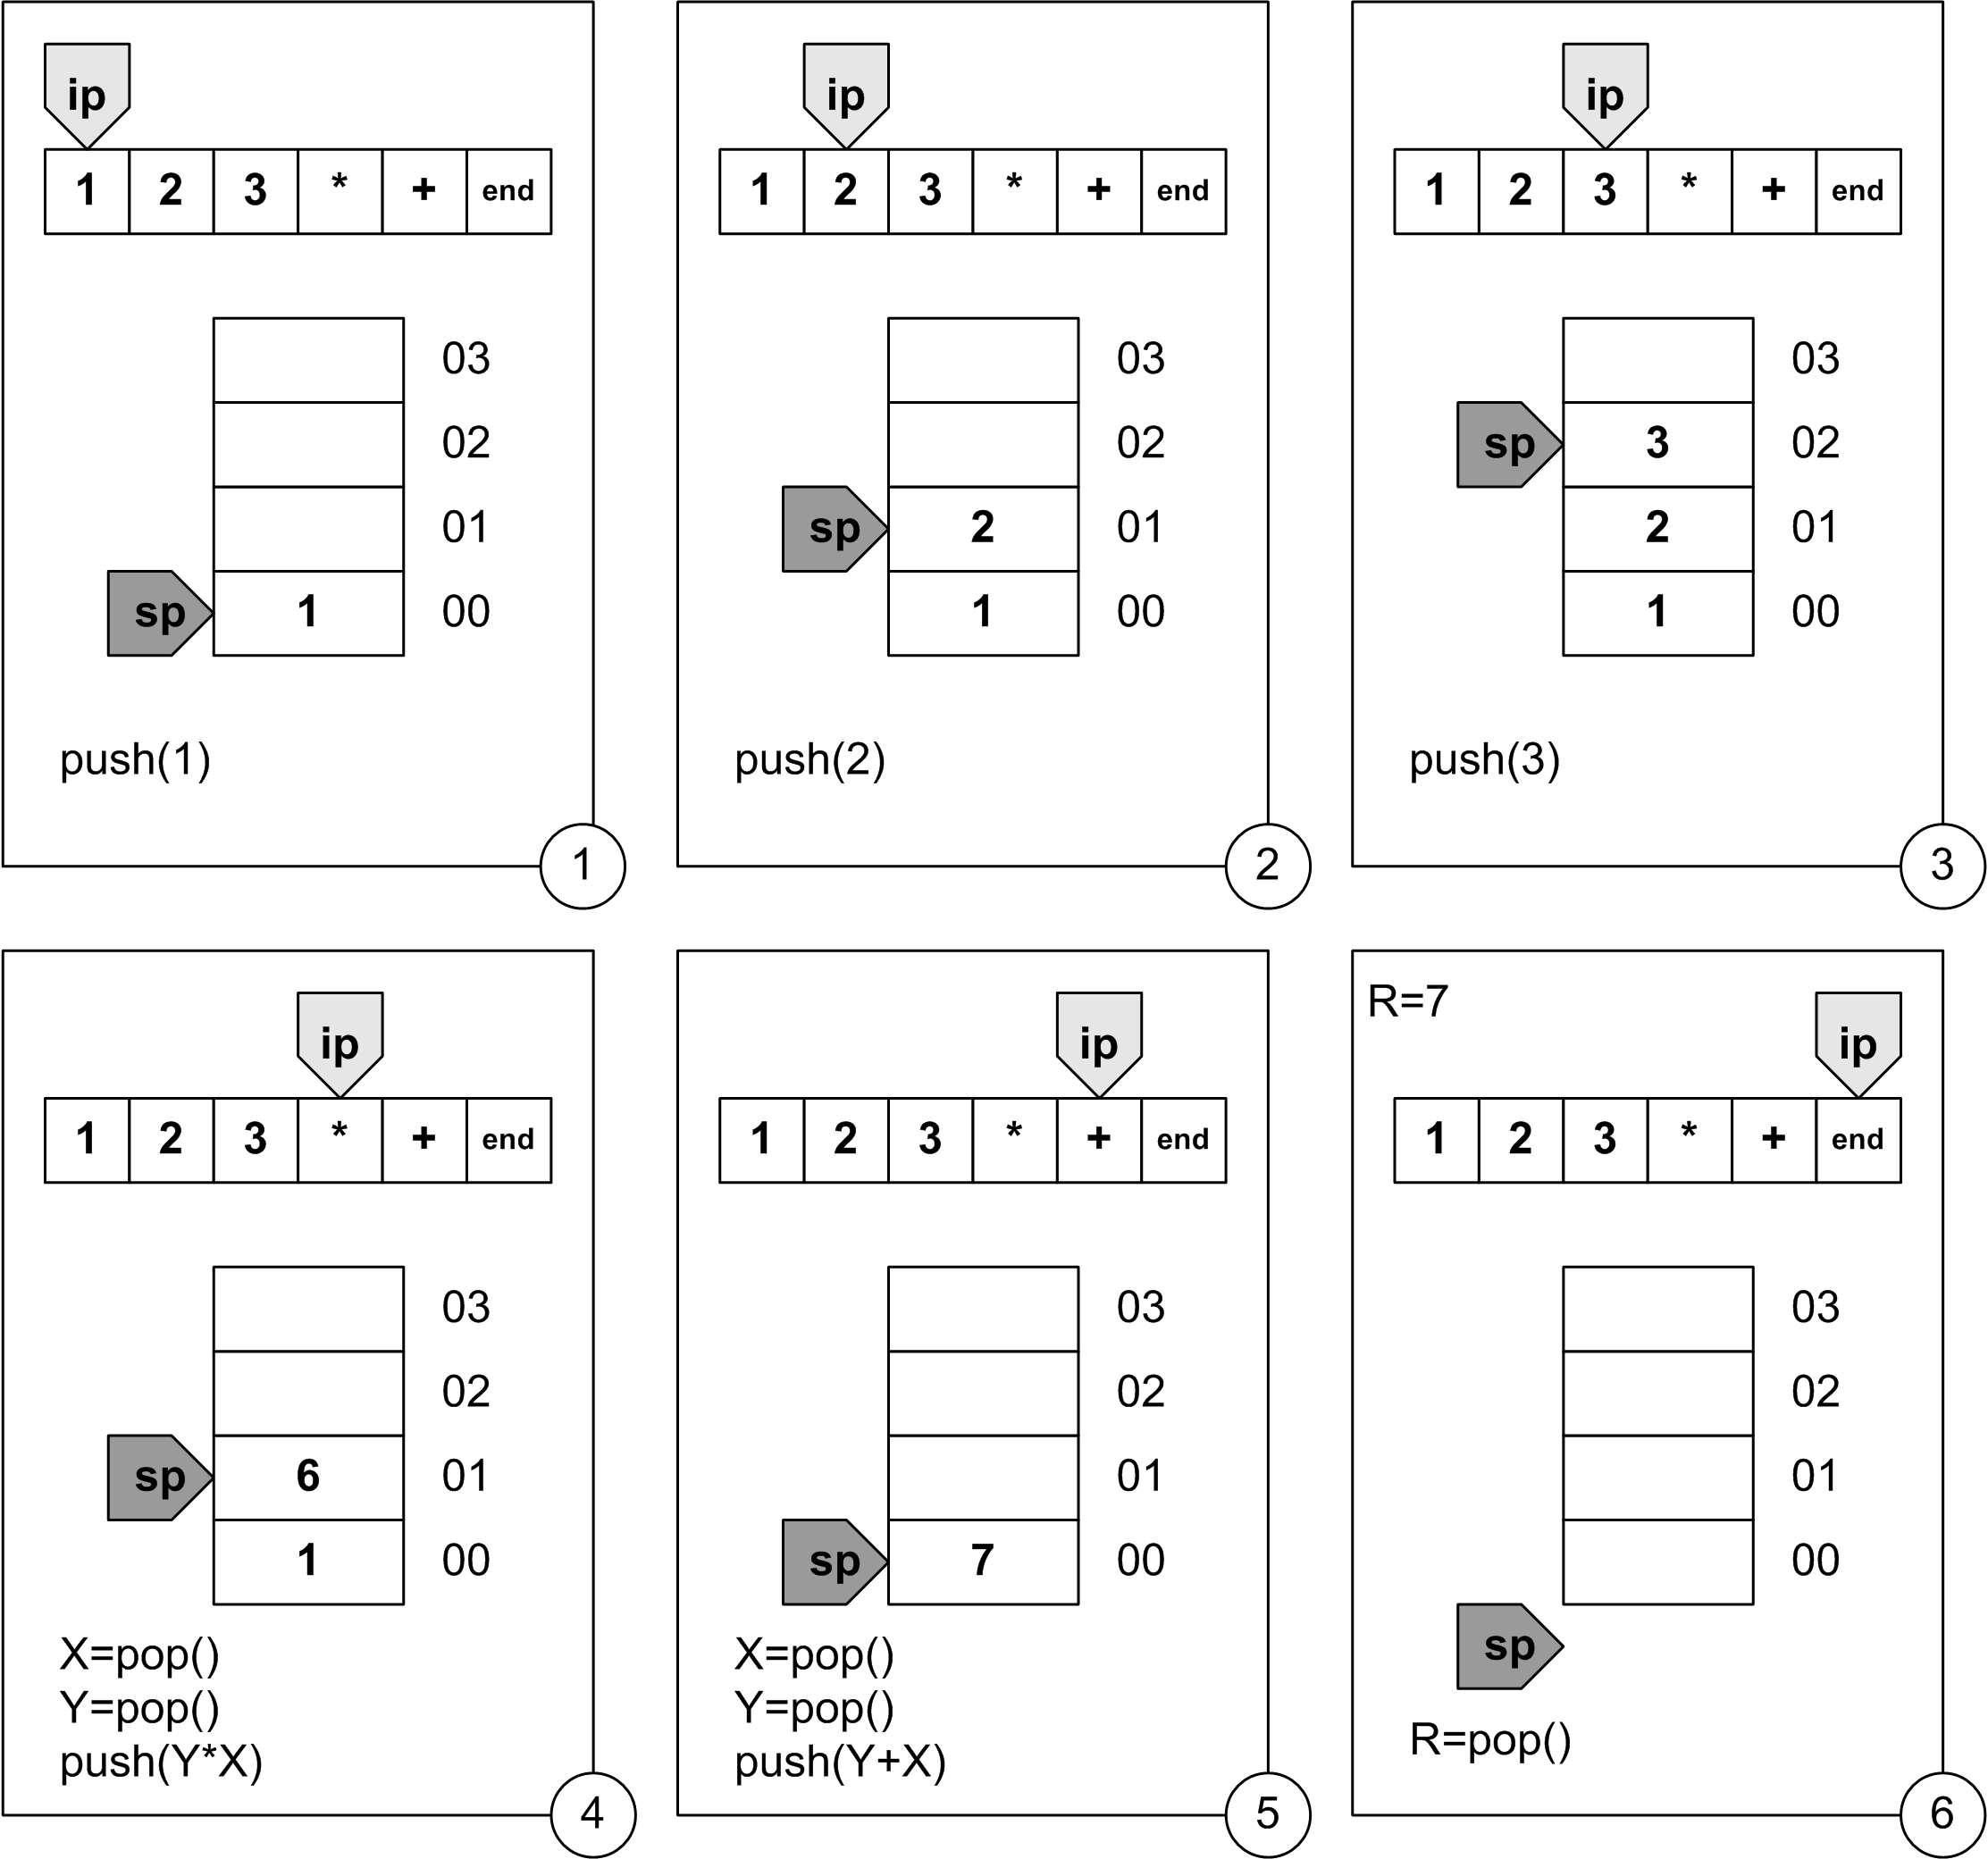
\includegraphics[width=0.6\textwidth]{fig/stackMachine.png}
    \]
\end{frame}



\appendix

\begin{frame}
    \frametitle{В заключение}
    
    Для углубленного изучения вопросов, касающихся индукции и рекурсии, рекомендуются книги \cite{bib:haggard:discrmathprogrammer,bib:miller:secParAlghorithm,bib:hopkroft:automateIntro}.    
\end{frame}


\begin{frame}[allowframebreaks]{Библиография}
    \bibliographystyle{gost780u}
    \bibliography{./../../bibliobase}
\end{frame}

\end{document}